\chapter{Conclusão}

A evolução do Mezuro não foi motivada por um motivo isolado. Um conjunto de fatores influenciaram e convenceram a equipe que o melhor para o futuro do projeto Mezuro seria um conjunto de modificações em sua estrutura. Os desenvolvedores estavam restritos aos ultrapassados recursos do Rails 2 e do Ruby 1.8, a qual não recebia mais suporte de seus desenvolvedores.

A equipe almejava por liberdade na tomada de decisões, como por exemplo atualizar o Mezuro para as novas versões do Rails e do Ruby, aproveitando suas melhorias e novos recursos. Porém, estavam subordinados as decisões e andamento do projeto Noosfero. A equipe se deu conta que os recursos relacionados a redes sociais fornecidos não eram necessários para uma ferramenta de monitoramento de código-fonte. Além disso, a manutenibilidade e inserção de novos desenvolvedores ao projeto eram tarefas difíceis, já que o Mezuro crescia bastante e se tornava cada vez mais uma aplicação dentro de outra aplicação, ao invés de um plugin com funcionalidades bem específicas.

Levando em conta todos esses fatores, a equipe do Mezuro decidiu retirá-lo do Noosfero, transformando-o em uma aplicação independente, além de formatar uma comunidade de software livre para atrair novos desenvolvedores. Para consolidar esses fatores, que levaram a evolução do Mezuro, foi elaborado um questionário (encontrado no Apêndice \ref{form-pesquisa}) direcionado e equipe que o mantém. Dos fatores que motivaram a evolução, os que mais foram citados pela equipe foram aqueles que limitam sua liberdade ou poder de decisão, que é o fato do Mezuro estar contido dentro do Noosfero, tendo seu desenvolvimento limitado.

É importante destacar que, embora o Mezuro esteja evoluindo para uma aplicação distinta do Noosfero, haverá uma integração, ainda a ser discutida pela comunidade de desenvolvedores, entre essas duas ferramentas futuramente.

\section{Contribuições}

A contribuição deste trabalho inclui os seguintes tópicos relacionados a implementação do Mezuro:
\begin{enumerate}
\item ``Manter Repositórios'';
\item ``Manter Configurações'';
\item Melhorias na composição de Configurações, ou seja, o fluxo de adição de métricas de configuração, assim como a edição das mesmas;
\item Adequação da identidade visual, de acordo com as melhores práticas relacionadas à usabilidade;
\item Aplicação de uma técnica de visualização de software;
\end{enumerate}

Os aspectos relevantes deste trabalho não estão restritos apenas aos  pontos práticos ou de implementação citados. A colaboração com um software livre, de acordo com os padrões de contribuição destacados na seção \ref{sec-padroes-sl}, passando por vários dos processos\footnote{Implementação, gerencia de configuração, requisitos e manutenção e evolução de software} que compõem a engenharia de software, além da aplicação de princípios ágeis\footnote{\textit{Pair programming}, divisão de iterações em \textit{sprints}, definição das unidades de trabalho dentro de \textit{backlog}}, interação e envolvimento com uma equipe remota também são pontos notáveis deste trabalho.

%
A técnica aplicada para a inserção do ciclo de usabilidade foi implementada seguindo as práticas de usabilidade para software livre proposto na dissertação de mestrado de Ana Paula Oliveira dos Santos. O grupo de desenvolvimento era composto por 15 membros, divididos em 8 membros da equipe Core, 5 co-desenvolvedores e 2 usuários ativos. Dentro do trabalho realizado foram abordadas todas as fases propostas de forma completa ou parcial das práticas de usabilidade para software livre.

\begin{itemize}
\item Identificar necessidades para design centrado em humano: Membro da equipe de desenvolvimento com foco em usabilidade a fim de coletar requisitos de tarefas e necessidades dos usuários;
\item Especificar contexto de uso: Realizado através de reuniões diárias e no planejamento da interação. As práticas definidas foram: Criar protótipos de tela, Coletar métricas (variáveis dependentes), Apresentar resultados das análises dos testes e Definição de histórias de usabilidade baseadas nos requisitos fornecidos pelos clientes
e no resultado dos testes de usuário;
\item Especificar requisitos: Testar protótipos com avaliações heurísticas;
\item Avaliar designs: Testar a usabilidade de protótipos com usuários locais e remotos (manipulação de variáveis independentes)
\end{itemize}

Os resultados obtidos através dos métodos de avaliação heurística, questionário PSSUQ e Checklist foram descritos na subseção \ref{evolucao-usabilidade}. Levando em consideração todos esses resultados realizado anteriormente foi possível observar uma melhoria progressiva com as interações de usabilidade sem impactar fortemente na rotina da equipe do projeto. As contribuições foram tanto em nível de \textit{front-end} quanto de \textit{back-end} e os membros com o foco de usabilidade participaram ativamente do desenvolvimento do código-fonte do projeto sem gerar nenhum tipo de deadlock. Isso possibilitou uma melhoria da usabilidade dentro da evolução de uma ferramenta da comunidade de software livre sem uma desestruturação de uma equipe tradicional das comunidades livres e sem a necessidade de gastos adicionais com uma equipe externa.  

\subsection{Limitações}
O código presente no apêndice \ref{radar-chart-code}, referente a técnica de visualização aplicada, o gráfico do radar, se encaixa bem na solução atual que o Mezuro fornece para o processamento de repositórios, que é o processamento de um repositório a cada instante. Porém é desejável que seja apresentado ao usuário o resultado de um ou mais processamentos, para possíveis comparações. Para a visualização dos resultados de mais de um processamento a solução atual não é satisfatória dado que os dados são lidos de um arquivo de extensão \textit{.tsv} onde não é possível separar os dados em grupos que representariam os resultados de cada processamento.

A avaliação de satisfação de usabilidade não pôde ser aplicada aos usuários devido ao fato da plataforma Mezuro estar em um ciclo de desenvolvimento (melhoria) e apesar de estar acessível\footnote{Plataforma Mezuro: http://mezuro.org/}, não é possível completar um ciclo de utilização devido ao módulo de análise do código estar em estado de refatoração em uma mudança de linguagem java para Ruby on Rails.

A quantidade de tecnologias envolvidas para geração de uma nova funcionalidade ou melhoria de um módulo gera uma deadline de aprendizado numa primeira contribuição ao projeto. Porem essa dificuldade é minimizada com a colaboração da equipe para a disseminação de conhecimento.

\subsection{Continuação}
As funcionalidade e melhorias realizadas no projeto possuem um intuito de continuidade e propagação dos seus benefícios ao longo de outras interfaces pela comunidade da plataforma Mezuro. O padrão gerado na primeira interação foi utilizado por desenvolvedores externos da equipe core a fim de aplicar o comportamento em outras telas que não sofreram a interação conforme citado na subseção \ref{evolucao-usabilidade}. O comportamento dinâmico e com a diminuição de fluxo da funcionalidade Configuration deverá ser aplicado nas funcionalidades \textit{New Project}, \textit{New Configuration} e \textit{New Repository}, por necessitarem de um comportamento similar. Enquanto a visualização, essa deverá ser aplicada para as métricas do projeto ao termino da fase de melhoria de desempenho da análise de código conforme na subseção \ref{visualizacao-software}. Com o termino dessas aplicações, a contribuição dessas melhorias deverá afetar diretamente ou indiretamente aproximadamente 80\% da interface da plataforma.

\subsection{Trabalhos Futuros}
Pensando em deixar uma perspectiva de trabalhos com foco em usabilidade para uma possível nova interação da comunidade Mezuro uma nova avaliação heurística foi realizada com foco em levantar pontos de melhoria. Os pontos de melhorias levantados foram
\begin{itemize}
\item Feedback ao usuário fixo

Os \textit{feedbacks} implementados na plataforma conforme Figura \ref{feedback}, modificam a estrutura da tela dificultando ao usuário o que diz respeito a facilidade de memorização, algumas das mensagens necessitam ser encerradas e com o acumulo dessas mensagens o agrupamento e a legibilidade da tela vai se perdendo.

\graphicspath{{figuras/}}
\begin{figure}[h]
\centering
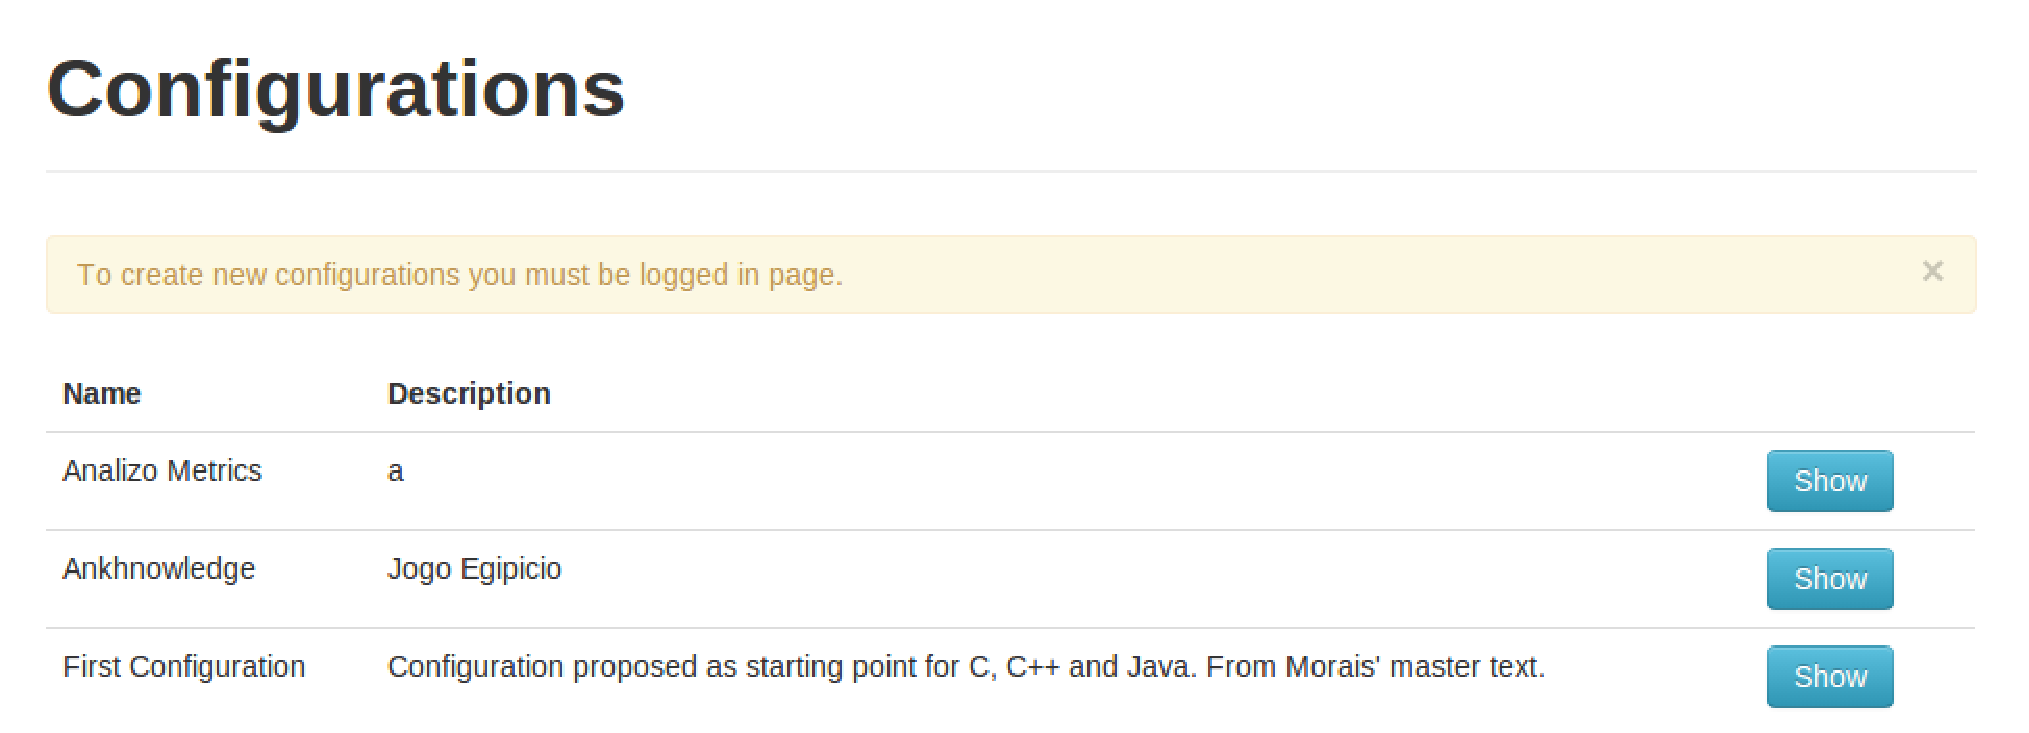
\includegraphics[width=1.0\textwidth]{FeedBack}
\caption{Feedback ao usuário}
\label{feedback}
\end{figure}

O esperado seria mensagens que não alterasse o agrupamento e legibilidade da tela, sem necessitar uma interação do usuário para encerramento dessas mensagens, tendo uma exibição limitada pelo tempo;

\item Feedback com tempo mínimo 

Os \textit{feedbacks} que não são fixos na tela apresentam tempo inapropriado, pois estão baseados no tempo de processamento das funcionalidades, em um máquina com maior processamentos as mensagens praticamente não são percebidas e a leitura delas não são possíveis. Esse tempo deve ser prefixado para um tempo médio da leitura da mensagem;

\item Internacionalização da plataforma

A plataforma Mezuro é apresentada totalmente na língua inglesa, por ser uma língua amplamente conhecida, porém há uma necessidade de se possibilitar a criação de internacionalização para que a comunidade possa desenvolver dicionários das mensagens em outras línguas e assim aumentar a abrangência do software.

\end{itemize}

As contribuições realizadas neste trabalho possuem relativa relevância dada a crescente força adquirida por projetos de software livre, principalmente o Mezuro que visa auxiliar a melhoria da qualidade de códigos-fonte. A metodologia aplicada a essas contribuições também merecem destaque já que foram aplicadas práticas ágeis que são cada vez mais utilizadas no desenvolvimento de software, e de vários processos que são objeto de estudo da engenharia de software.

A distância entre as equipes dos laboratório Lappis - FGA/UnB e CCSL - IME/USP poderia se tornar um grande empecilho ao desenvolvimento e colaboração da equipe da UnB ao Mezuro. Porém a comunicação, uma característica que é priorizada pelos métodos ágeis, supriu essa desvantagem através das reuniões semanais e grupo de emails ativo.

A comunicação entre os membros das equipes é importante em vários aspectos. Entre eles está a aplicação de padrões durante o desenvolvimento, os quais impactam diretamente na manutenibilidade do sistema. Segundo \citeauthor{pigoski1996practical} o esforço para compreensão de programas ou documentos (código-fonte), compreende cerca de 47\% a 62\% do esforço total de desenvolvimento de um software. Essa afirmação ficou clara durante as contribuições com o Mezuro, principalmente no início, onde a tecnologia era pouco conhecida pelos membros da equipe da UnB. Porém, conforme a tecnologia se tornava mais familiar aos desenvolvedores e a interação e  comunicação entre as equipes se tornava maior, o esforço para compreensão diminuía, o que era auxiliado também pela característica da linguagem Ruby, que favorece a manutenibilidade, dada sua legibilidade.